% !TEX root = deliverable1.3.tex




%% !TEX TS-program = pdflatex
%\documentclass{article}
%
%\usepackage{hl_short}
%\usepackage{times}
%\usepackage{graphicx}
%\usepackage{latexsym}
%
%\usepackage{bm}
%\usepackage{amsbsy}
%\usepackage{amsmath}
%\usepackage{amsfonts}
%\usepackage{amssymb}
%
%\usepackage{subfigure}
%\usepackage{color}
%
%\usepackage{theorem}
%
%\theoremstyle{theorem}
%\newtheorem{theorem}{Theorem}
%
%\usepackage{array}
%
%\theoremstyle{definition}
%\newtheorem{definition}{Definition}
%\newtheorem{remark}{Remark}
%
%\newcommand{\bu}[1]{\mathbf{#1}}
%\newcommand{\bv}[1]{\bm{#1}}
%
%
\newcommand{\W}{\mathbf{W}}
\newcommand{\X}{\mathbf{X}}
\newcommand{\Y}{\mathbf{Y}}
\newcommand{\Z}{\mathbf{Z}}
\newcommand{\w}{\mathbf{w}}
\newcommand{\x}{\mathbf{x}}
\newcommand{\y}{\mathbf{y}}
\newcommand{\z}{\mathbf{z}}
\newcommand{\argmax}[1]{\underset{#1}{\operatorname{arg}\,\operatorname{max}}\;}

%\newcommand{\comment}[1]{ \begin{center}{\bf [[ #1 ]]}\end{center}}
%
%\title{Practical Considerations for Testing the Cajamar Use Case}
%\author{Sigve, Helge, Thomas, Ana, Ramon, Antonio}
%\date{\today}
%
%
%\begin{document}
%\maketitle
%

\section{Cajamar: Test and evaluation}

This section introduces the testing procedures for the Cajamar use cases. 
It builds on the general principles for evaluation already described in the previous sections of this report, and exemplifies how these principles can be employed in the setting of the credit evaluation application scenarios. 

\subsection{Use-case requirements}

The test and evaluation procedures for Cajamar will be developed along the lines introduced in Deliverable 2.1 (D2.1): Instead of testing each use case separately, we utilize the notion of {\em application scenarios}. 
An application scenario is defined by a sequence of use cases that combined constitutes a full interaction procedure leading to a verifiable result. In D2.1 we defined two scenarios:

\bde
\item[CAJ1: Prediction probability of default:]
The application scenario covers the first five use cases  defined in Deliverable 1.2 (D1.2):
\bit 
\item UC1: Data reading and attribute construction
\item UC2: Feature selection
\item UC3: Model construction
\item UC4: Model application
\item UC5: Result checking and risk update
\eit

\item[CAJ2: Low risk profile extraction:] This application area uses the same model that is developed in the first scenario, but then progresses to use the model differently. It covers the following use cases:
\bit 
\item UC1: Data reading and attributes construction
\item UC2: Feature selection
\item UC3: Model construction
\item UC6: Profile extraction
\eit
\ede

Requirements for the different use-cases were defined in D1.2. Most requirements are functional in nature, but some also introduce hard requirements that can be tested quantitatively. The latter are repeated in \tabref{cajamar:requirements} for completeness. We note that the requirements center around three issues:
\ben
\item The whole process covered by Application scenario CAJ1, starting with SQL queries and ending with report generation must take less than 3 hours for the 5.6M clients (requirements CAJ.U1.O1, CAJ.U2.O1, CAJ.U4.D1, CAJ.U4.O1, and CAJ.U5.O1).
\item The prediction quality for Application scenario CAJ1, evaluated by AUROC, must be higher than $90\%$ (CAJ.U3.D3).
\item The quality of the profiles generated in Application scenario CAJ2 is required to improve the benefit of at least $5\%$ (CAJ.U6.O3).
\een

\begin{table}
\scalebox{.89}{

\begin{tabular}{|p{16mm}|p{17mm}|p{100mm}|p{12mm}|}\hline
ID & Sub-phase & Description & Task(s)\\ \hline\hline
CAJ.U1.O1&	Interface 	&SQL queries should be efficient enough so that the whole process takes less than 3 hours.	&	8.2\\ \hline
CAJ.U2.O1& 	Interface	&The feature selection should be efficient enough so that the whole process takes less than 3 hours. & 4.3\\ \hline
CAJ.U3.D3&	Testing	&AUROC should be higher than $90\%$. & 8.3\\\hline
CAJ.U4.D1&	Develop.	&Model application should be efficient enough so that the whole process takes less than 3 hours. &2.3, 3.3, 4.1, 4.4\\\hline
CAJ.U4.O1&	Testing	&Model should be able to evaluate daily about 5.6M clients.	&	2.3, 3.3, 4.1, 4.2\\\hline
CAJ.U5.O1&	Interface 	&The risk data update process should be efficient so that the whole process takes less than 3 hours. & 8.2\\\hline
CAJ.U6.O3&	Testing	&Expected benefits of a marketing campaign using obtained profiles should be $5\%$ higher than with current methods. & 8.3\\
\hline \hline\end{tabular}

}
\caption{Testable requirements for the Cajamar use-cases.}\label{tab:cajamar:requirements}
\end{table}





\subsection{Model and data characteristics}

%\comment{The following is from D2.1. Some slight adaptions, as I have removed all about the ``Evaluation set''. Should be made more to the point?}


\subsubsection{The data generation process}

Both application scenarios use the same dataset, containing the defaulting behaviour of the Cajamar clients\footnote{The second application scenario will use only a subset of the total number of features.}. We now briefly describe the data generation process (the description is adapted from D2.1, where a more comprehensive description can be found). Please refer to \figref{CajaMarTimeLineReduced} for the timeline. 


\begin{figure}[ht!]
\centering
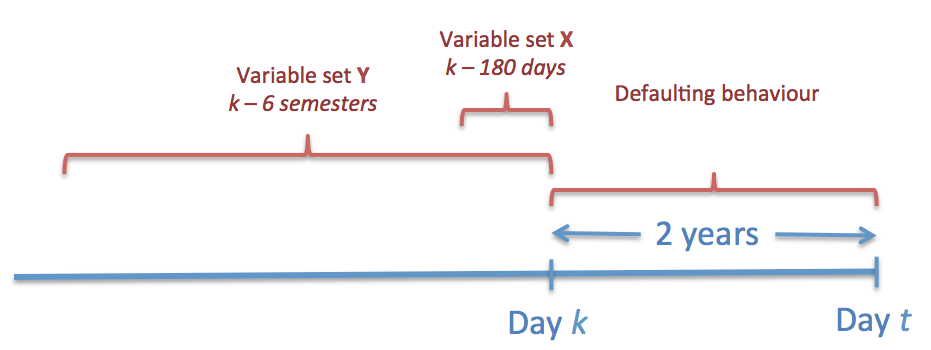
\includegraphics[scale=0.35]{figures/CajamarTimeLineReduced}
\caption{\label{fig:CajaMarTimeLineReduced}Time-line showing the generation of the data set. $t$ refers to the present time and $k$ corresponds to time $t-2$\ years. There are two disjoint groups of variables, denoted as $\X$ and $\Y$, with different past information considered, $180$ days back (daily) and $6$ semesters back (aggregated by semester), respectively.}
\end{figure}


The dataset is created at time $k$,  and contains a record for every client to be evaluated. 
Predictive variables refer here to the financial activity and payment behaviour of the customers in recent past as well as to their socio-demographic information, which usually does not change over time. 

Attributes denoted by $\X$ refer to the financial activity  during the last 180 days. Examples of these features include ``account balance'' and ``number of credit card operations''. 
They usually change daily for a customer and are encoded by introducing a set of variables for each attribute -- one for each day back from time $k$. 
Hence, the financial activity of a customer is specified by a number of variables equal to 180 times the number of attributes. 

For others attributes, denoted by $\Y$, we are interested in information from the last $36$ months. Examples of variables in this set include payments inside Cajamar (loans, mortgages, credits, etc.). 
The information from the last 36 months is grouped by semester, giving $6$ summary variables per attribute that is considered. 
Finally, there are some static variables (mainly encoding socio-demographic aspects) denoted by $\Z$. These are not included in \figref{CajaMarTimeLineReduced} as they are not time-indexed. 

The objective of the data analysis is to detect if a customer with profile $(\X,\Y,\Z)$ will default within the next two years. This corresponds to the class label in the dataset, \textit{Defaulter}, and is determined by inspecting the user's behaviour from time $k$ and $2$ years into the future, i.e., in the period from $k$ to $t$ (see \figref{CajaMarTimeLineReduced}). We obtain this information directly from Cajamar's databases simply by selecting the time $k$ to be two years back in time, and thereby letting $t$ be the current time. Note that, at the present time (time $t$), we have information of the \textit{Defaulter} variable in the period of time from $k$ to $t$. Thus,  Defaulter$^{(k)}$ indicates if at some point in this period the customer was a defaulter.

The format of the data set for training/updating the model is depicted in \tabref{TrainingDataset}. Each record contains the values for all predictive variables and a class variable. The class variable is labelled as \emph{non-defaulter} only when there is no defaulting in the period from $k$ to $t$ (2 years). 
\begin{table}[ht!]
\centering
\begin{tabular}{c|ccc|ccc|c|c}
	&\multicolumn{3}{c|}{Days} & \multicolumn{3}{c|}{Semester} & \\
     Time $t$              & $\X^{(k-180)}$ & $\ldots$ & $\X^{(k-1)} $ & $\Y^{(k-6)}$  & $\ldots$ & $\Y^{(k-1)} $ & $\Z$ & Defaulter$^{(k)}$\\  
\hline
Client$_1$  &                                                  &              &                     &                               &                     &        &  \\ 
$\vdots$      &                                                 &               &                     &                                &                     &       & \\ 
Client$_n$  &                                                &               &                     &                                &                     &     & \\ 
\end{tabular} 
\caption{Three groups of attributes $\X$, $\Y$ and $\Z$ are distinguished according to the past information required. Current time is denoted as $t$. The data set is built at time $t$ with $k=t - 2$ years. }
\label{tab:TrainingDataset} 
\end{table}

\subsubsection{The generated dataset}

The existing data set was generated at $t$ equal to December 31$^\text{st}$ 2013, thus simulating the calculations as if the AMIDST system was run two years before that ($k$ corresponds to December 31$^\text{st}$ 2011). 
The dataset includes all customers who have been a client of Cajamar in the period  $k$ and up to day $t$, corresponding to $n=4.5\text{M}$ customers. 

Every member of the dataset has been classified as either non defaulter or defaulter (no missing entries). 
Customers can have missing attribute values in their description. In particular, some of the clients were not clients in the whole three year period before day $k$. If a customer was not associated to Cajamar at some point in time $k - 6 \mbox{ semesters}$, there will be missing values for some of the variables in $\Y^{(k-6)}$. 
 %RAMON: This is not true. I therefore deleted the statement. NB! Inconsistency with D2.1, where we say it is so.
 % However, Cajamar will manually fill in all relevant missing values using other data sources. 
%Formally, every member $i$ of the dataset therefore has a vector of explanatory variables denoted by $\W_i=\{ \X_i^{(k-180)}, \ldots, \X_i^{(k-1)}, \Y_i^{(k-6)},\ldots, \Y_i^{(k-1)},\Z_i\}$ without missing values. In total, each customer is described using $7036$ variables.
Formally, every member $i$ of the dataset  has a vector of explanatory variables denoted by $\W_i=\{ \X_i^{(k-180)}, \ldots, \X_i^{(k-1)}, \Y_i^{(k-6)},\ldots, \Y_i^{(k-1)},\Z_i\}$, potentially with some missing values (encoded using special codes). 
In total, each customer can be described using $7036$ variables, that is, $180\sizeof{\X} + 6\sizeof{\Y} + \sizeof{\Z} = 7036$, where $\sizeof{\cdot}$ is the number of variables in each group.

Of all the customers in the dataset, $76\%$ are considered to be of no risk because they do not have a loan in the bank, approximately $20\%$ of the customers were exposed but did not default, and $3.79\%$ of the customers  defaulted in the two-year period of interest. 

This data set will be used both for training and testing purposes. The test-set is defined by randomly selecting $20\%$ of the customers. For reproducibility, a documented procedure including a fixed random seed is used to select the customers in the test set. 




\subsection{Predictive performance: test and evaluation}


\subsubsection{Application scenario 1}

The goal of the first application scenario is to determine if a customer is going to be a defaulter after two years. This corresponds to a classification problem, where the class variable is denoted as Defaulter$^k$ in \tabref{TrainingDataset}. 

The approach of the AMIDST project is to calculate $r_i=P(\mbox{Default}_i^k \,|\, \w_i)$ for each customer $i$. These quantities update the risk table in the system (see Table~\ref{tab:riskTable}).
If, at some point, the probability of default of a customer rises above a predefined threshold, the bank may take preventive actions to reduce the risk of defaulting by this customer.

\begin{table}[ht!]
\centering
\begin{tabular}{c|ccc|ccc|c}
     Time $t$  & Risk of being defaulter \\  
\hline
Client$_1$  &    $r_1$  \\ 
$\vdots$      &   $\vdots$   \\ 
Client$_n$  &   $r_n$  \\ 
\end{tabular} 
\caption{Risk for the bank customers where $r_i$ represents the probability of being defaulter for customer $i$.}
\label{tab:riskTable}
\end{table}



According to requirement CAJ.U3.D3, the risk prediction quality should be assessed using the area under the receiver operating characteristic (ROC) curve. 
The classification rule is that a customer $i$ is classified as a defaulter if $r_i \geq C$ for some constant $C$, and the ROC curve is computed by  plotting the rate of true positives against the rate of true negatives for various choices of $C$.  The requested area can then be found directly, and should, according to the requirement, be larger than $0.90$ (see also \secref{hypothesisSpace}).

There are two main issues with the outlined approach:
\bde
% RAMON: this is not a problem. The AMIDST system will only be used for monitoring customers who have already been granted a loan, not for the grant-decision in itself
%\item[Relevance of the data:]  All the customers' data made available to the project for training and testing belong to people already associated with Cajamar, and their economic status (e.g., regarding whether or not they have obtained a loan) is a consequence of Cajamar's current system being employed to remove the customers not deemed appropriate. The dataset we have access to may therefore not reflect the distribution of customers that approach Cajamar in the first place (and which AMIDST will be exposed to if employed in production).

\item[Changes in the economic climate:]  A Cajamar customer's chance of defaulting is to some  extent determined by external factors, like the economic climate in Spain. During the economic crisis, the rate of defaulters was significantly higher than what was observed prior to the onset of the crisis. The data set we work with, corresponds to the period of the crisis, and it is natural to expect that the relationships found by the model are optimized for that economic climate. The AUC criteria is chosen to remedy global effects that affect all customers in a similar way, but we can still not guarantee that the model will perform at a similar level for a fundamentally different economic climate. In some cases these differences in the economic climate might be overcome by some of the socio-economic variables, for instance, a civil servant's personal economy with a permanent job should be less influenced by the economic climate than a casual/seasonal worker.

\item[Stable versus volatile climate:] Customers in the training and test sets are per definition from the same time period. Learning from the training data, we will therefore be able to detect the economic climate to which the customers will be exposed (e.g., simply by detecting the fraction of defaulters in the training data). If put in production, the predictions the  AMIDST model is asked to make will be about the future, i.e., shifted two years in time when compared to the training data. This is not a problem if the economic climate is static or only slowly varying, but will be disastrous if, for instance, AMIDST is asked to make predictions about future customers immediately before the onset of a new economic crisis.

\ede

To partly account for these shortcomings of the test procedure we have collected another dataset with $k$ equal to December 31$^\text{st}$ 2013, and where the correct class labels will be discovered two years later (December 31$^\text{st}$ 2015).
As of today, the class labels for this dataset are unknown, but will be supplied at the end of 2015, and will  therefore be available for the formal testing in Task 8.3. 
An AUC of more than $90\%$ when using this new dataset for testing (and the original dataset for training) would be seen as a strong indication of the applicability of AMIDST in production.






\subsubsection{Application scenario 2}




Currently, a marketing campaign in Cajamar involves two steps:
\begin{itemize}
 \item The first step is conducted by the marketing department, and results in a list of candidate customers. 
The list contains clients that have a high probability of signing what is offered to them (for instance a credit card).  
\item The second step, conducted by the risk modellers, is to filter out clients that are risky in terms of defaulting.
\end{itemize} 

The task described in Use case 4 is to find relevant users profiles. The profiles can, for instance, be used to conduct marketing campaigns. The profiles should contain customers that are likely to be non-defaulters, and cover only attributes that are found to be relevant by the domain experts. It is required (CA.U6.O3) that the expected benefits of a marketing campaign using the obtained profiles should be $5\%$ higher than with current methods.  

Direct quantitative evaluation of the AMIDST-generated profiles is difficult to perform in a formal way mainly for two reasons. The first reason is that the application scenarios generate a \textit{user profile} and not a \textit{set of users}. 
We cannot value a profile in itself; it is the application of the profile to generate user sets that can potentially be monetized. The second reason is that the AMIDST profile defines users that are not likely to default, not users that are likely to sign a contract (and therefore not necessarily users who are valuable as marketing objects). For instance, it seems natural to expect the AMIDST profile to prefer solvent customers living in their own homes without any mortgage and with a sizeable cash-account. On the other hand, a customer like that may not be relevant to target for a campaign selling small-sized cash-loans without security requirements. This leads to a two-tier evaluation of the profiles, first considering the profiles as generators of profitable marketing campaigns, next as a way to evaluate the ability to find customers that will not default.


\begin{description}
\item [1) EVALUATION OF A CAMPAIGN'S PROFIT:]  
Cajamar currently uses theoretical measurements for evaluating marketing campaigns. Let $s_i=P(\mbox{Signs}_i \,|\, \w_i)$ be the probability that a customer $i$ signs on an offer presented to him (calculated by an existing system used by Cajamar) and, as before, let $r_i=P(\mbox{Default}_i^k \,|\, \w_i)$ be the probability that customer $i$ defaults on a loan within the next two years (given that the offer is accepted). Furthermore, let $\gamma_i$ be the net present value for the bank of that offer given that the customer does not default, and  $\Gamma_i$ the cost of the offer if a customer ends up in defaulting. $c$ is a fixed indirect cost of the campaign. Then, the loss of a customer would be
\begin{equation}
 L(\w_i,s_i,r_i) = \left\{\begin{array}{ll}
 s_i r_i\Gamma_i +   (1-s_i) (1-r_i)\gamma_i + c& \text{ if a loan is offered;} \\
s_i (1-r_i)\gamma_i  & \text{ otherwise.} \\ \end{array}\right.   \label{equ:cajamarTheoretical}
 \end{equation}


We therefore propose that the profile extraction is evaluated as follows:

\ben
\item A marketing campaign is selected, and the set of customers contacted are listed. The set of customers is called $\calC$.
\item The AMIDST system is used to generate a profile for non-defaulting customers, and a fixed number of  customers fitting the profile (comparable to the number of elements in $\calC$) are selected.
 The marketing department selects a subset of the customers in this set based on their probability to contract. Call this reduced set of customers $\calA$. Note that the set $\calA$ now defines a fictitious campaign (chosen by AMIDST) and has not been employed in a real campaign. 
\item The two sets $\calC$ and $\calA$ are compared qualitatively and quantitatively (using the theoretical measure in \equref{cajamarTheoretical}).
\een
In \equref{cajamarTheoretical} all customers that are not included in the campaign will contribute with the loss $s_i (1-r_i)\gamma_i$. In practice, contributions will only be collected from the set of customers that is selected by either method, i.e., the set of customers in $\calC\cup\calA$ because a customer selected by neither system (i.e., not in $\calC\cup\calA$) will  contribute equally to the loss of each method, and is therefore not helpful to establish the difference between them. 

\item [2) EVALUATION OF DEFAULTING BEHAVIOUR:]

A drawback of this approach is that the loss-function rests upon (theoretical) probabilities $P(\mbox{Default}_i^k \,|\, \w_i)$ and $P(\mbox{Signs}_i \,|\, \w_i)$. Due to the introduction of $P(\mbox{Signs}_i \,|\, \w_i)$ in the loss function, we cannot in general guarantee that the system that is best at predicting the defaulting behavior will obtain the lowest loss. 
To target the quantitative requirement without using the theoretical probabilities we therefore also propose to utilize the AMIDST risk prediction capability from application Scenario 1 directly in the marketing setting, where the following procedure will be performed:
\bit
\item Select a historical marketing campaign that is at least two years old, and remove all customers that did not sign. The remaining set of customers is called $\calC$.
\item  Filter out clients that the AMIDST system deem too risky. The set of customers is called $\calA$. Note that $\calA\subseteq\calC$.
\item Calculate the empirical loss of the set $\calA$ compared to that of $\calC$. The requirement is that the loss of $\calA$ should be at least $5\%$ lower than the loss of the set $\calC$. Note that for a direct comparison, only the difference in the two sets,  $\calC\setminus\calA$, will contribute, and the costs of applying the AMIDST solution will be $\gamma_i$ for the customers that do not default and $-\Gamma_i$ for those that do. 
\eit
It should be noted that this procedure only evaluates the AMIDST system's ability to remove poor customers from the list of customers that were included in the original campaign, as we are unable to quantify the effect of AMIDST potentially wanting to send marketing material to customers that were not selected for the historical campaign without using the theoretical construct of \equref{cajamarTheoretical}.  The two evaluation approaches must therefore be seen in combination to give the full picture.

\end{description}

\vekk{




\comment{Rest of the section is Sigve's text. I propose that we remove all the math into the start-up-sections and just use established stuff like ``Empirical risk'' here. Not sure if all of Sigve's points have been included in the ``for dummies'' - version I have written. Must be checked.}



There are more opportunities with testing the second step.  After performing step one the test data set is reduced to a set of clients with a high contracting probability (i.e. above a certain level).  Let the clients in this data set be $(x_i, y_i)$, where $y_i$ is either default or not default and $x_i$ is a vector of explanatory variables.  It makes sense to compute AUC for both the current method and the Amidst method to compare the two methods.  This comparison will say something about the ability of the filter to take out defaulters, while keeping the non defaulters.  However, we must assume that the real probability of contracting $P(\bv{x_i})$ is completely independent of whether the client will actually default or not.

Moreover, in Delivery 1.2, it is required that the benefit of a AMIDST induced marketing campaign should be more than 5 percent higher than a normal campaign.  In order to discuss such a requirement we have to iintroduce a function that describes the financial loss of a certain classification rule compared to a classification rule that make no mistakes. 

In this paper, we define the \emph{loss function} as a real and lower-bounded function $L(x_i, h(x_i), y_i)$. It takes into account the explanatory variables for each client $x_i$, the predicted class $h(x_i)$ and the true class label $y_i$. 

In the current system in Cajamar the classification rule is denoted $h_{\mbox{Current},L_1}$ and is defined by

\begin{equation}
\label{def:empRisk}
h_{\mbox{Current},L_1}(x_i) = P_{\mbox{Current}}(\mbox{Default}_i \,|\, \bv{x_i}) \leq L_1 
\end{equation}
where the probability for defaulting client $i$ are $P_{\mbox{Current}}(\mbox{Default}_i \,|\, \bv{x_i})$.  Here, $L_1$ is a chosen classification limit. 

We let the cost of excluding client $i$ that does not default as $c_i(0|1)$ and also the cost of including client $i$ that does default as $c_i(1|0)$.  Both costs are related to the size of the potential offer.  Also, we make the assumption that the real probability of contracting $P(\bv{x_i}) = p$ is completely independent of whether the client will actually default or not.  The loss function below is of interest

\begin{equation}
\label{def:empRiskBank}
L(x_i, h_{\mbox{Current},L_1}(x_i) , y_i) = 
\begin{cases}
0     &\quad \mbox{for} \quad h_{\mbox{Current},L_1}(x_i) = 0 \quad \& \quad y_i = 0\\
p c_i(1|0)    &\quad \mbox{for} \quad h_{\mbox{Current},L_1}(x_i) = 1 \quad \& \quad y_i = 0\\
p c_i(0|1)      &\quad \mbox{for} \quad h_{\mbox{Current},L_1}(x_i) = 0 \quad \& \quad y_i = 1\\
0   &\quad \mbox{for} \quad h_{\mbox{Current},L_1}(x_i) = 1 \quad \& \quad y_i = 1.
\end{cases}
\end{equation}
Notice that $L$ is an array of $n \times 2\times 2$ elements. Cajamar can estimate $c_i(0|1)$ and $c_i(1|0)$ for all clients in the database.

The empirical risk is found by averaging the loss function on the training set given by 

\begin{equation}
\label{def:empRisk}
R_{emp}(h_{\mbox{Current},L_1}, \bv{x}) = n^{-1} \sum_{i=1}^n L(x_i, h_{\mbox{Current},L_1}(x_i), y_i).
\end{equation}

It is now possible to calculate the empirical risk involved with using both the current filter and also the Amidst filter.  It is therefore possible to estimate the ratio between the costs and therefore see whether there is more than 5 percent gain in using the Amidst default filter compared to using the current default filter.  Notice that in terms of estimating this gain percentage it is not needed to estimate $p$.  However, it could be estimated from the number that accepted the offer on an old campaign.


\subsubsection*{Calculating empirical risk on an old campaign}

It is also possible to use an old campaign to test the improvement of using the Amidst default filter in addition to the current filter. 

Consider an old campaign that was done more than two years ago. Even though costs and default/non defaults are known for all clients, the loss function is only known on the clients that was targeted in that campaign.  This makes this discussion complicated. 

We will now consider the AMIDST induced marketing campaign as a binary classification problem with class variable $y_i$, which can take the values $\{0,1\}$. Class one refers to non-defaulters that actually signs the contract and class zero refers to the rest of the clients.  In a perfect campaign only the non-defaulters that actually signs the offer (for instance a credit card or a loan) are selected.  

In the current system in Cajamar the classification rule is denoted $h_{\mbox{Current},L_1,L_2}$ and is defined by

\begin{equation}
\label{def:empRisk}
h_{\mbox{Current},L_1,L_2}(x_i) = P_{\mbox{Current}}(\mbox{Default}_i \,|\, \bv{x_i}) \leq L_1 \, \& \,P_{\mbox{Current}}(\mbox{Contract}_i \,|\, \bv{x_i}) \geq L_2,
\end{equation}
where the probability for defaulting and contracting for client $i$ are $P_{\mbox{Current}}(\mbox{Default}_i \,|\, \bv{x_i})$ and $P_{\mbox{Current}}(\mbox{Contract}_i \,|\, \bv{x_i})$.  Here, $L_1$ and $L_2$ are chosen classification limits. 

We let the cost of excluding client $i$ that actually would contract and not default as $c_i(0|1)$.  This cost is related to the size of the potential offer.

Moreover, we let $c_i(1|0)$ be the cost of offering to client $i$, provided that he either would not take the offer or would default if he took the offer.  Clearly, if client $i$ was offered and contracted but defaulted, $c_i(1|0)$ is related to the size of the contract.  Otherwise, $c_i(1|0)$ is only related to the cost of making the offer.  The loss function below is of interest

\begin{equation}
\label{def:empRiskBank}
L(x_i, h_{\mbox{Current},L_1,L_2}(x_i) , y_i) = 
\begin{cases}
0     &\quad \mbox{for} \quad h_{\mbox{Current},L_1,L_2}(x_i) = 0 \quad \& \quad y_i = 0\\
c_i(1|0)    &\quad \mbox{for} \quad h_{\mbox{Current},L_1,L_2}(x_i) = 1 \quad \& \quad y_i = 0\\
c_i(0|1)      &\quad \mbox{for} \quad h_{\mbox{Current},L_1,L_2}(x_i) = 0 \quad \& \quad y_i = 1\\
0   &\quad \mbox{for} \quad h_{\mbox{Current},L_1,L_2}(x_i) = 1 \quad \& \quad y_i = 1.
\end{cases}
\end{equation}

Cajamar can estimate $c_i(0|1)$ and $c_i(1|0)$ for all clients in the database.


The empirical risk for the old campaign is not taking into account the financial loss related to excluding a number of clients that actually would have contracted and not defaulted.  Said with other words, the empirical risk is not taking into account losses related to when $h_{\mbox{Current},L_1,L_2}(x_i) = 0$, and $y_1 = 1$.  In such a calculation none of the $c_i(0|1)$s are used.  The empirical risk will therefore be less than the true risk (which would take the above point into account).

A simple test is to use the Amidst toolbox to provide an additional filter related to default prediction on top of the old classification rule.  Mathematically this is

\begin{equation}
\begin{split}
\label{eq:filter}
h_{\mbox{Amidst filter},L_1,L_2,L_3}(x_i) = &
P_{\mbox{Current}}(\mbox{Default}_i \,|\, \bv{x_i}) \leq L_1
 \, \& \,
P_{\mbox{Current}}(\mbox{Contract}_i \,|\, \bv{x_i}) \geq L_2
\, \& \,  
\\ &
P_{\mbox{Amidst filter}}(\mbox{Default}_i \,|\, \bv{x_i}) \leq L_3.
\end{split}
\end{equation}
This calculation of empirical risk is biased by the same amount as the old method.  It makes therefore sense to compare $R_{emp}(h_{\mbox{Amidst filter},L_1,L_2,L_3}, \bv{x}) $ with $R_{emp}(h_{\mbox{Current},L_1,L_2}, \bv{x}) $.
The benefit of using the Amidst model as additional filter can therefore be quantified.

\subsection*{Questions: }
\begin{enumerate}
\item Do you see any flaw in reasoning?
\item What more should we do?
\item What do you think about the profiling ideas?
\end{enumerate}


}

\subsection{Run-time performance: test and evaluation}
\subsubsection{Application scenario 1}

According to the requirement procedure, the full process starting with SQL statements and ending with validation of the new risks should be completed in no more than three hours (CAJ.U1.O1, CAJ.U2.O1, CAJ.U4.D1, CAJ.U5.O1).

The AMIDST solution will be installed in a server (IBM System x3690 X5) with the following characteristics:
\bit
\item 2 Intel Xeon 10C Processors (Model E7-2870 130w 2.40GHz/30MB)
\item 256GBRAM,16x16GB(1x16GB,4Rx4,1.35V)PC3L-8500CL7ECCDDR3
1066MHz LP RDIMM
\item 2 internal disks SAS �IBM 146 GB 2.5in SFF Slim-HS 15K 6Gbps SAS HDD� RAID, one of them �hot swap�. 10 Disks IBM 600GB 2.5in SFF 10K 6Gbps HS SAS HDD.
\eit
This server is mainly used by credit risk models and marketing models departments. Data will be obtained via SQL queries. The current Information Center database management system is Oracle, but is being changed to a Teradata solution.

Learning the AMIDST model, however, requires an iterative process that is performed until convergence, and whose number of steps, and hence time, might vary due to random initialization. One way to enforce that the 3 hour upper bound is not violated, is to specify a \textit{timeout} counter for the learning algorithm. Ideally, there should be enough time for the learning algorithm to reach convergence, and the timeout counter should be only included as a safe mechanism.

In order to provide a reliable estimation of the average time employed by the learning process and its expected performance, the following two graphs will be plotted:
\begin{itemize}
\item A first graph whose $x$-axis shows the number of tests and $y$-axis the total time employed by each of the experiments. Apart from the mean, a confidence interval at e.g. a $99\%$ confidence level, will be provided to guarantee that the expected time will be included among this interval with a margin of error of $1\%$. 
\item A second graph in which the $x$-axis corresponds to the number of iterations/time and $y$-axis to the performance of the learning algorithm (indicating how close it is to convergence, e.g. lower bound in variational Bayes). 
\end{itemize}

Joint interpretation of the two graphs will give us knowledge about the expected running time and performance of the process. We want to provide a mechanism to ensure that with a level of confidence of $99\%$, the learning algorithm will converge at the desired time limit. In the worst case, the algorithm will provide a valid outcome that might not be optimal.  
Note that the same analysis should also be performed for any other stochastic algorithms utilized in the process of the application scenario.


\vekk{
\comment{Testing procedure/how strictly we will look at this must be evaluated.
\bit 
\item What happens if we finish only 95\% of the customers? RAMON: We need 100\%. 
\item Will there be variations in the run-time e,g, do to other users of the system? RAMON: Yes!. However, cannot state how much load the server will have. Solution?
\item Is the *max* time required to be less than 3hrs, median, \ldots RAMON: Max
\item Scalability through more hardware if we fail to meet the three hrs demand? RAMON: This is an option, but not for the short time-span
\eit

To me, this seems under-specified. If the system is using 99\%\ of the resources elsewhere we cannot get all the customers done in 3 hrs., but this is what he wants?

}
}


\subsubsection{Application scenario 2}

There are no specific run-time requirements for this application scenario. Specifically, it is stated that \textit{``[\ldots] execution time of this process is not relevant because the marketing campaigns are not launched so frequently.''}.



\vekk{

\newpage




%% This part written by Sigve. I'm keeping it here for reference (and copy-paste'ing. Rewrite to conform with the new layout of the document. 
%% This work initiated by Helge Langseth on Nov 20th 2014

There are two application scenarios here.  The first one is prediction of whether a client will default within two years or not and the second is related to the benefit of a marketing campaign. For clarity we have added the description about the data set from delivery 2.1 without any modification.

\section{Description from 2.1}

%-------------------------------------------------------------------------------------------------------
\subsection{Predicting probability of default} \label{SubSection:Predicting}
%-------------------------------------------------------------------------------------------------------

Our objective is to tackle the current limitations of the risk prediction problem by \textit{daily} learning the predictive model and also updating the risk of default for every bank customer. Dependences among the variables will now be considered, as well as including all the variables in the analysis. With these changes, Cajamar plans to improve the quality of the prediction model by increasing the area under ROC curve significantly.


Therefore, the process will consist in building a \textit{training set} as well as a set of customers to be evaluated, called \textit{evaluation set} (see Deliverable 1.2~\cite{Fer14b}). How these data sets are generated gives us some insights into the nature of this risk prediction problem (see Figure~\ref{Figure:CajaMarTimeLine} for a better understanding):

%Next, we detail how these data sets are collected .
%Figure~\ref{Figure:CajaMarTimeLine} illustrates how both evaluation and training data sets are collected within a time-line. The current time is denoted as $t$ and the time $2$ years back as $k$, i.e., $k=t-2$ years. 

\begin{figure}[ht!]
\centering
\includegraphics[scale=0.35]{figures/CajamarTimeLine}
\caption{\label{Figure:CajaMarTimeLine}Time-line showing the generation of the evaluation (in green) and training (in red) data sets. $t$ refers to the present time and $k$ corresponds to time $t-2$\ years. Both in the training and test data sets, there are two disjoint groups of variables, denoted as $\X$ and $\Y$, with different past information considered, $180$ days back (daily) and $6$ semesters back (by semester), respectively.}

\end{figure}

\begin{itemize}

\item \textbf{Model evaluation data set:} This data is created at time $t$ and contains a record for every client to be evaluated. Note that information about the predicted defaulting behaviour is missing at time $t$ and it will be obtained after performing inference on the model. Predictive variables refer here to the financial activity and payment behaviour of the customers in recent past as well as to their socio-demographic information which usually does not change over time. 

There are attributes, denoted as $\X$, for which information during the last 180 days is considered. 
%recent \textcolor{red}{{\bf financial activity}}of a customer refers to attributes such as ``account balance'', ``number of credit card operations'', etc. stored in the last 180 days. 
These attributes usually change daily for a customer, so they are encoded by introducing a set of variables for each attribute, one for each day back from the current time $t$. Hence, the financial activity of a customer is specified by a number of variables equal to 180 times the number of attributes. For others attributes, denoted as $\Y$, we are interested in information from the last $36$ months grouped by semester. 
%In the case of \textcolor{red}{{\bf past payment behaviour}}, the attributes refer to variables related to \textcolor{red}{payments inside Cajamar (loans, mortgages, credits, etc.).} Information from the last 36 months grouped by semester is considered for these variables. 
Therefore, similar to previous group of variables, $6$ variables for each of these attributes will be considered. Finally, there are some other static variables, denoted as $\Z$, not included in Figure~\ref{Figure:CajaMarTimeLine} as they are not indexed over time. The data set for the evaluation of customers is depicted in Table~\ref{tab:EvaluationDataset}. 


%with information about \textcolor{red}{payments to other financial institutions or companies (phone and electricity bills, public bodies, etc.)} 
%are included in this group of variables. They are denoted as .

%The group of variables denoted as $\Z$ mainly includes socio-demographic variables and they are not indexed over time as they remain fixed.  

\begin{table}[ht!]
\centering
\begin{tabular}{c|ccc|ccc|c}
	&\multicolumn{3}{c|}{Days} & \multicolumn{3}{c|}{Semester} \\
     Time $t$              & $\X^{(t-180)}$ & $\ldots$ & $\X^{(t-1)} $ & $\Y^{(t-6)}$  & $\ldots$ & $\Y^{(t-1)} $ & $\Z$  \\  
\hline
Client$_1$  &                                                  &              &                     &                               &                     &        \\ 
$\vdots$      &                                                 &               &                     &                                &                     &      \\ 
Client$_n$  &                                                &               &                     &                                &                     &     \\ 
\end{tabular}
\caption{Evaluation data set at time $t$ for all the clients. Three groups of attributes $\X$, $\Y$ and $\Z$ are distinguished according to the past information required. Current time is denoted as $t$.}
\label{tab:EvaluationDataset} 
\end{table}

Thus, the objective is to compute the probability of defaulting within the following two years of each record from the evaluation data set, and afterwards update the risk table in the system (see Table~\ref{tab:riskTable}).

\begin{table}[ht!]
\centering
\begin{tabular}{c|ccc|ccc|c}
     Time $t$  & Risk of being defaulter \\  
\hline
Client$_1$  &    $r_1$  \\ 
$\vdots$      &   $\vdots$   \\ 
Client$_n$  &   $r_n$  \\ 
\end{tabular} 
\caption{Risk table for the bank customers where $r_i$ represents the probability of being defaulter for customer $i$.}
\label{tab:riskTable}
\end{table}

If, at some point, the probability of default of a customer rises above a predefined threshold, the bank may take preventive actions to reduce the risk of defaulting by this customer.


\item \textbf{Model training data set:}  This data set is also built at time $t$ in a similar way as the evaluation data. It contains the same set of features as well as the target variable \textit{Defaulter} but with information referred to time $k$ instead (two years back). Note that, at time $t$, we have information of the \textit{Defaulter} variable in the period of time from $k$ to $t$. Thus,  Defaulter$^{(k)}$ indicates if at some point in this period she/he was a defaulter.

The data set for training/updating the model is depicted in Table~\ref{tab:TrainingDataset}.
\begin{table}[ht!]
\centering
\begin{tabular}{c|ccc|ccc|c|c}
	&\multicolumn{3}{c|}{Days} & \multicolumn{3}{c|}{Semester} & \\
     Time $t$              & $\X^{(k-180)}$ & $\ldots$ & $\X^{(k-1)} $ & $\Y^{(k-6)}$  & $\ldots$ & $\Y^{(k-1)} $ & $\Z$ & Defaulter$^{(k)}$\\  
\hline
Client$_1$  &                                                  &              &                     &                               &                     &        &  \\ 
$\vdots$      &                                                 &               &                     &                                &                     &       & \\ 
Client$_n$  &                                                &               &                     &                                &                     &     & \\ 
\end{tabular} 
\caption{Training data set built at time $t$ with $k=t - 2$ years.  The notation for predictive variables is the same as in Table~\ref{tab:EvaluationDataset}.}
\label{tab:TrainingDataset} 
\end{table}

Table~\ref{tab:TrainingDataset} shows the training data set where each record contains the values for all predictive variables and a class value labelled as \emph{non-defaulter} only when there is no evidence of defaulting in the period from $k$ to $t$ (2 years). 

\end{itemize}

\section{Test and evaluation regime}

The training set above is actually the data set that we are going to train on and also test on. This may be a source to confusion, but from now on the training set above will be defined as the dataset and the evaluation set is not even considered in relation to testing. 

The only criterion for being a member of the dataset is that the member has been a client continuously from day $k$ and up to day $t$.  Every member of the dataset has a class label that is either non defaulter or defaulter.  There are no missing values related to class labels.  However, there are missing values related to attributes.  In particular, some of the clients where not clients in the whole three year period before day $k$.  Cajamar will manually fill in all relevant missing values.  Formally, every member $i$ of the dataset has a vector of explanatory variables that is denoted by $\bv{x_i} =\{ \X_i^{(k-180)},  \X_i^{(k-1)}, ...\Y_i^{(k-6)}, \Y_i^{(k-1)},\Z_i\}$.  

We will divide this data set into a training set and a test set by a completely random process.

\subsection{Requirements for the first use case scenario: default prediction}

In the first use case scenario, it is required that the AUROC should be above 0.90.
 
The Bayesian network basically computes the probability $P(\mbox{Default}_i \,|\, \bv{x_i})$ and the classification rule is
$P(\mbox{Default}_i \,|\, \bv{x_i}) \geq C$.  The ROC curve is computed by basically plotting the rate of true positives against the rate of true negatives for various choices of $C$.  AUROC is the area under the graph.  (There is also another way of computing AUROC which do not involve computing the rate of true positives and rate true negatives for various $C$, but this is omitted in this discussion.)

\subsubsection*{Questions: }
\begin{enumerate}
\item How many defaulters and non defaulters do we have on both the training set and the test set?
\item Can you go though all the information and make sure that it is correct.
\end{enumerate}


\subsection{Requirements for the second use case scenario:  AMIDST induced marketing campaign}

A marketing campaign in Cajamar involves two steps.  The first step is to find clients that have a high probability of signing what is offered (for instance a credit card).  The second step is to filter out clients that are risky in terms of defaulting.
The testing regime involves testing each step separately.

The first step is difficult to test. We suggest that the Amidst profiler finds a list of a certain number of clients that are manually inspected by the marketing department in Cajamar. This list can for instance be compared to a list of clients with high contracting probability from a former campaign.

There are more opportunities with testing the second step.  After performing step one the test data set is reduced to a set of clients with a high contracting probability (i.e. above a certain level).  Let the clients in this data set be $(x_i, y_i)$, where $y_i$ is either default or not default and $x_i$ is a vector of explanatory variables.  It makes sense to compute AUC for both the current method and the Amidst method to compare the two methods.  This comparison will say something about the ability of the filter to take out defaulters, while keeping the non defaulters.  However, we must assume that the real probability of contracting $P(\bv{x_i})$ is completely independent of whether the client will actually default or not.

Moreover, in Delivery 1.2, it is required that the benefit of a AMIDST induced marketing campaign should be more than 5 percent higher than a normal campaign.  In order to discuss such a requirement we have to iintroduce a function that describes the financial loss of a certain classification rule compared to a classification rule that make no mistakes. 

In this paper, we define the \emph{loss function} as a real and lower-bounded function $L(x_i, h(x_i), y_i)$. It takes into account the explanatory variables for each client $x_i$, the predicted class $h(x_i)$ and the true class label $y_i$. 

In the current system in Cajamar the classification rule is denoted $h_{\mbox{Current},L_1}$ and is defined by

\begin{equation}
\label{def:empRisk}
h_{\mbox{Current},L_1}(x_i) = P_{\mbox{Current}}(\mbox{Default}_i \,|\, \bv{x_i}) \leq L_1 
\end{equation}
where the probability for defaulting client $i$ are $P_{\mbox{Current}}(\mbox{Default}_i \,|\, \bv{x_i})$.  Here, $L_1$ is a chosen classification limit. 

We let the cost of excluding client $i$ that does not default as $c_i(0|1)$ and also the cost of including client $i$ that does default as $c_i(1|0)$.  Both costs are related to the size of the potential offer.  Also, we make the assumption that the real probability of contracting $P(\bv{x_i}) = p$ is completely independent of whether the client will actually default or not.  The loss function below is of interest

\begin{equation}
\label{def:empRiskBank}
L(x_i, h_{\mbox{Current},L_1}(x_i) , y_i) = 
\begin{cases}
0     &\quad \mbox{for} \quad h_{\mbox{Current},L_1}(x_i) = 0 \quad \& \quad y_i = 0\\
p c_i(1|0)    &\quad \mbox{for} \quad h_{\mbox{Current},L_1}(x_i) = 1 \quad \& \quad y_i = 0\\
p c_i(0|1)      &\quad \mbox{for} \quad h_{\mbox{Current},L_1}(x_i) = 0 \quad \& \quad y_i = 1\\
0   &\quad \mbox{for} \quad h_{\mbox{Current},L_1}(x_i) = 1 \quad \& \quad y_i = 1.
\end{cases}
\end{equation}
Notice that $L$ is an array of $n \times 2\times 2$ elements. Cajamar can estimate $c_i(0|1)$ and $c_i(1|0)$ for all clients in the database.

The empirical risk is found by averaging the loss function on the training set given by 

\begin{equation}
\label{def:empRisk}
R_{emp}(h_{\mbox{Current},L_1}, \bv{x}) = n^{-1} \sum_{i=1}^n L(x_i, h_{\mbox{Current},L_1}(x_i), y_i).
\end{equation}

It is now possible to calculate the empirical risk involved with using both the current filter and also the Amidst filter.  It is therefore possible to estimate the ratio between the costs and therefore see whether there is more than 5 percent gain in using the Amidst default filter compared to using the current default filter.  Notice that in terms of estimating this gain percentage it is not needed to estimate $p$.  However, it could be estimated from the number that accepted the offer on an old campaign.


\subsubsection*{Calculating empirical risk on an old campaign}

It is also possible to use an old campaign to test the improvement of using the Amidst default filter in addition to the current filter. 

Consider an old campaign that was done more than two years ago. Even though costs and default/non defaults are known for all clients, the loss function is only known on the clients that was targeted in that campaign.  This makes this discussion complicated. 

We will now consider the AMIDST induced marketing campaign as a binary classification problem with class variable $y_i$, which can take the values $\{0,1\}$. Class one refers to non-defaulters that actually signs the contract and class zero refers to the rest of the clients.  In a perfect campaign only the non-defaulters that actually signs the offer (for instance a credit card or a loan) are selected.  

In the current system in Cajamar the classification rule is denoted $h_{\mbox{Current},L_1,L_2}$ and is defined by

\begin{equation}
\label{def:empRisk}
h_{\mbox{Current},L_1,L_2}(x_i) = P_{\mbox{Current}}(\mbox{Default}_i \,|\, \bv{x_i}) \leq L_1 \, \& \,P_{\mbox{Current}}(\mbox{Contract}_i \,|\, \bv{x_i}) \geq L_2,
\end{equation}
where the probability for defaulting and contracting for client $i$ are $P_{\mbox{Current}}(\mbox{Default}_i \,|\, \bv{x_i})$ and $P_{\mbox{Current}}(\mbox{Contract}_i \,|\, \bv{x_i})$.  Here, $L_1$ and $L_2$ are chosen classification limits. 

We let the cost of excluding client $i$ that actually would contract and not default as $c_i(0|1)$.  This cost is related to the size of the potential offer.

Moreover, we let $c_i(1|0)$ be the cost of offering to client $i$, provided that he either would not take the offer or would default if he took the offer.  Clearly, if client $i$ was offered and contracted but defaulted, $c_i(1|0)$ is related to the size of the contract.  Otherwise, $c_i(1|0)$ is only related to the cost of making the offer.  The loss function below is of interest

\begin{equation}
\label{def:empRiskBank}
L(x_i, h_{\mbox{Current},L_1,L_2}(x_i) , y_i) = 
\begin{cases}
0     &\quad \mbox{for} \quad h_{\mbox{Current},L_1,L_2}(x_i) = 0 \quad \& \quad y_i = 0\\
c_i(1|0)    &\quad \mbox{for} \quad h_{\mbox{Current},L_1,L_2}(x_i) = 1 \quad \& \quad y_i = 0\\
c_i(0|1)      &\quad \mbox{for} \quad h_{\mbox{Current},L_1,L_2}(x_i) = 0 \quad \& \quad y_i = 1\\
0   &\quad \mbox{for} \quad h_{\mbox{Current},L_1,L_2}(x_i) = 1 \quad \& \quad y_i = 1.
\end{cases}
\end{equation}

Cajamar can estimate $c_i(0|1)$ and $c_i(1|0)$ for all clients in the database.


The empirical risk for the old campaign is not taking into account the financial loss related to excluding a number of clients that actually would have contracted and not defaulted.  Said with other words, the empirical risk is not taking into account losses related to when $h_{\mbox{Current},L_1,L_2}(x_i) = 0$, and $y_1 = 1$.  In such a calculation none of the $c_i(0|1)$s are used.  The empirical risk will therefore be less than the true risk (which would take the above point into account).

A simple test is to use the Amidst toolbox to provide an additional filter related to default prediction on top of the old classification rule.  Mathematically this is

\begin{equation}
\begin{split}
\label{eq:filter}
h_{\mbox{Amidst filter},L_1,L_2,L_3}(x_i) = &
P_{\mbox{Current}}(\mbox{Default}_i \,|\, \bv{x_i}) \leq L_1
 \, \& \,
P_{\mbox{Current}}(\mbox{Contract}_i \,|\, \bv{x_i}) \geq L_2
\, \& \,  
\\ &
P_{\mbox{Amidst filter}}(\mbox{Default}_i \,|\, \bv{x_i}) \leq L_3.
\end{split}
\end{equation}
This calculation of empirical risk is biased by the same amount as the old method.  It makes therefore sense to compare $R_{emp}(h_{\mbox{Amidst filter},L_1,L_2,L_3}, \bv{x}) $ with $R_{emp}(h_{\mbox{Current},L_1,L_2}, \bv{x}) $.
The benefit of using the Amidst model as additional filter can therefore be quantified.

\subsection*{Questions: }
\begin{enumerate}
\item Do you see any flaw in reasoning?
\item What more should we do?
\item What do you think about the profiling ideas?
\end{enumerate}

}

%
%
%\bibliographystyle{named}
%\bibliography{ijcai13}
%
%\end{document}
%
